\chapter{Architektur des OpenVC Compilers}
{\em 
In diese Kapitel wird die Architektur erl�utert, dynamische sowie statische. Es wird dabei erkl�rt wie VHDL Source Code durch den OpenVC Compiler verarbeitet wird.
}
\section{Statische und dynamiche Architektur}
\subsection{Phasen}
Der Compiler verarbeitet den Source Code in vier verschiedenen Phasen
\begin{figure}
  \centering
    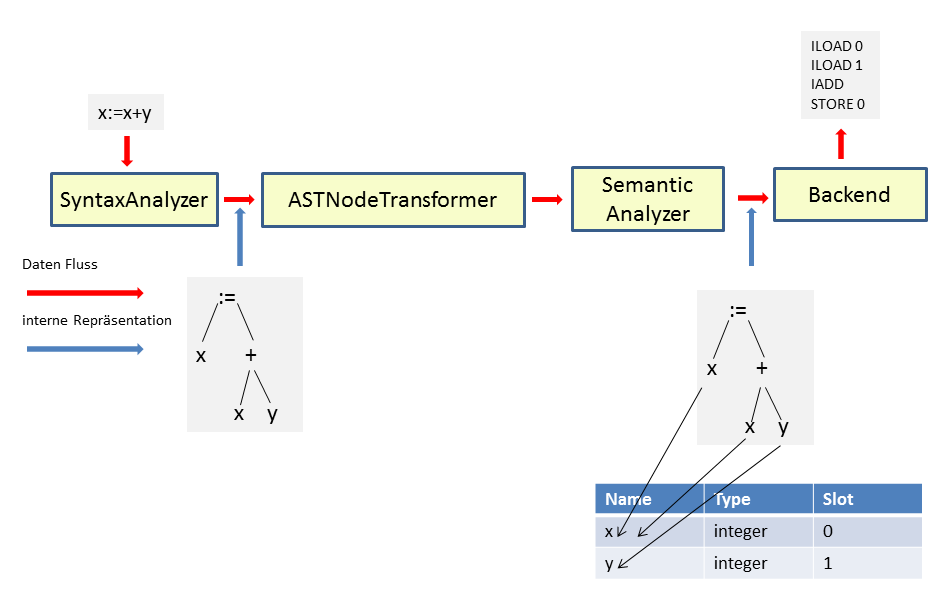
\includegraphics[scale=0.7]{images/CompilerPhasen.png}
    \caption{Die vier Phasen des Compiler}
\end{figure}

\subsection{Klassen�bersicht}
\todo{Text}
\section{Scanner/Parser mit Antlr}
\begin{quotation}
Eine Grammatik hei�t LL(1) (d.h. analysierbar von links nach rechts mit linkskanonischen Ableitungen und einem Vorgriffssymbol), wenn an jeder Stelle, an der man zwischen mehreren Alternativen w�hlen kann, gilt, dass die terminalen Anf�nge dieser Alternativen paarweise disjunkt sind. Mit anderen Worten: Der Parser muss jederzeit mit einem einzigen Vorgriffssymbol entscheiden k�nnen, welche von mehreren m�glichen Alternativen er w�hlen soll. \cite{moess}
\end{quotation}

Die im Standard \cite{ieee} beschriebene Syntax liegt bereits in Extended Backus-Naur Form (EBNF) \cite{wirth} vor, weist aber einige LL(1) Konflikte auf, die vorher behoben wurden.
In der Beschreibung von Coco/R [M�ss03] werden drei verschiedene M�glichkeiten erl�utert, wie diese Konflikte gel�st werden k�nnen. Mit Hilfe dieser drei Varianten ist es auch gelungen, die Grammatik in eine f�r Antlr valide LL(1) Form umzuwandeln. Die drei Ans�tze zur Behebung der Konflikte werden nachstehend erl�utert.

\subsection{Faktorisierung}
Bei der Faktorisierung werden gemeinsame Teile herausgezogen und an den Anfang der Produktion gestellt. Z.B. kann die folgende Produktion
\begin{center} A = a b c | a b d. \end{center} 
in die Produktion A'
\begin{center} A' = a b (c | d). \end{center} 
ohne Konflikte umgewandelt werden.
\todo{Beispiel}
%\lstset{caption={}}
%\lstinputlisting[style=ANTLR]{src/test.g}

\subsection{Umwandlung in Iterationen}
Linksrekursion stellt in LL(k) Sprachen im Gegensatz zu LR basierten immer ein Problem dar. In der Produktion
\begin{center} A = A b | c. \end{center} 
starten beide Alternativen mit c. Durch eine Umwandlung der Rekursion in eine Iteration kann dieses Problem gel�st werden, z.B wird die Produktion A zu
\begin{center} A' = c \{b\}. \end{center}
\todo{Beispiel}
\subsection{Einsatz von \textit{Conflict Resolvers}}
Bei dem Einsatz von \textit{Conflict Resolvers} kann unterschieden werden, wie viele Tokens der Parser vorausschauen muss, um eine Entscheidung zu treffen.

\subsubsection{Konstante Anzahl von \textit{Lookahead Tokens}}
Diese F�lle k�nnten meistens auch durch den Einsatz von Faktorisierung gel�st werden, aber die Lesbarkeit der Grammatik w�rde darunter leiden. Durch die Ber�cksichtigung von mehreren Tokens in die Entscheidung verh�lt sich der Parser effektiv wie ein LL(k) basierter.
\todo{Beispiel}

\subsubsection{Unbekannte Anzahl von \textit{Lookahead Tokens}}
Hier muss der Parser beliebig viele Tokens konsumieren und wird dabei in einen LL(*) basierten umgewandelt. [Par07]
\todo{Beispiel}

\section{AST}
\subsection{AST Konstruktion}
\todo{Text}

\subsection{AST Beispiel}
Im folgenden Abschnitt wird anhand von konkreten Beispielen genauer verdeutlich, wie der konstruierte AST im Speicher dargestellt wird, wobei die einzelnen Kanten der Graphen die Variablen der verschiedenen Klassen darstellen. Es wird zuerst immer der entsprechende Programmcode gezeigt und anschlie�end der entsprechende Graph mit den AST-Knoten.

\subsubsection{WhileStatement}
\lstset{caption={},language=VHDL}
\lstinputlisting{src/WhileStatement.vhd}
\begin{figure}
  \centering
    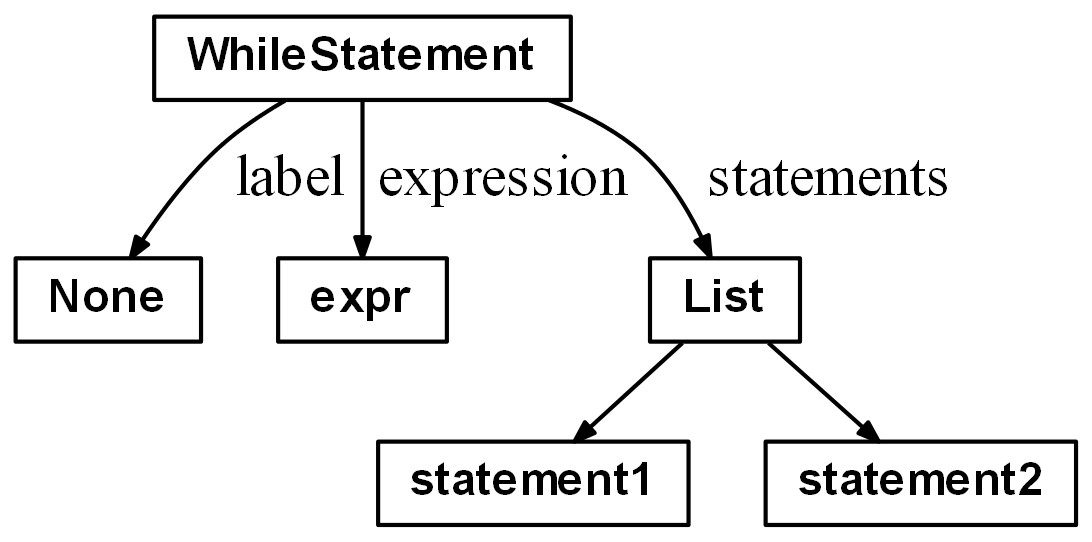
\includegraphics[scale=0.6]{images/WhileStatement.png}
    \caption{AST-Knoten f�r ein While-Statement}
\end{figure}
Ein While-Statement besteht aus einer Expression, die in der Variable \textit{expression} gespeichert wird und einer Liste von Statements die in \textit{statements} gespeichert werden.

\subsubsection{IfStatement}
\lstset{caption={}}
\lstinputlisting{src/IfStatement.vhd}
\begin{figure}
  \centering
    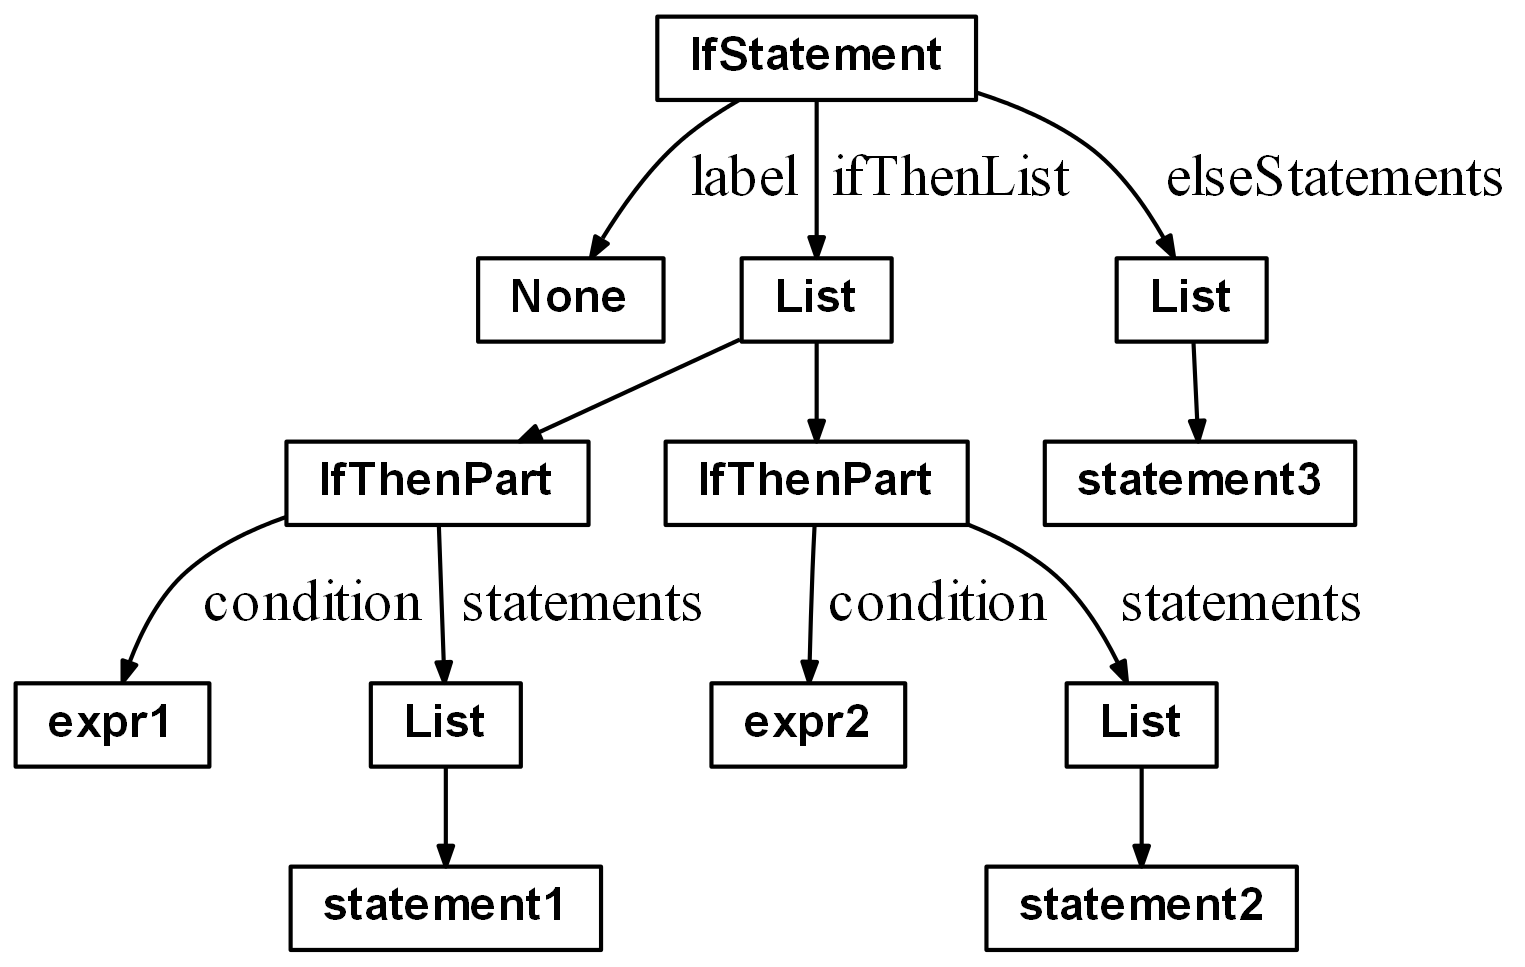
\includegraphics[scale=0.6]{images/IfStatement.png}
    \caption{AST-Knoten f�r ein While-Statement}
\end{figure}
Ein If-Statement besteht aus mehreren Zweigen, wobei die einzelnen Zweige Instanzen der Klasse IfThenPart sind, wo die Condition und die Liste der Statements gespeichert werden. Die Variable elseStatements enth�lt die Statements aus dem else-Zweig.

\subsubsection{LogicalExpression}
\lstset{caption={}}
\lstinputlisting{src/LogicalExpression.vhd}
\begin{figure}
  \centering
    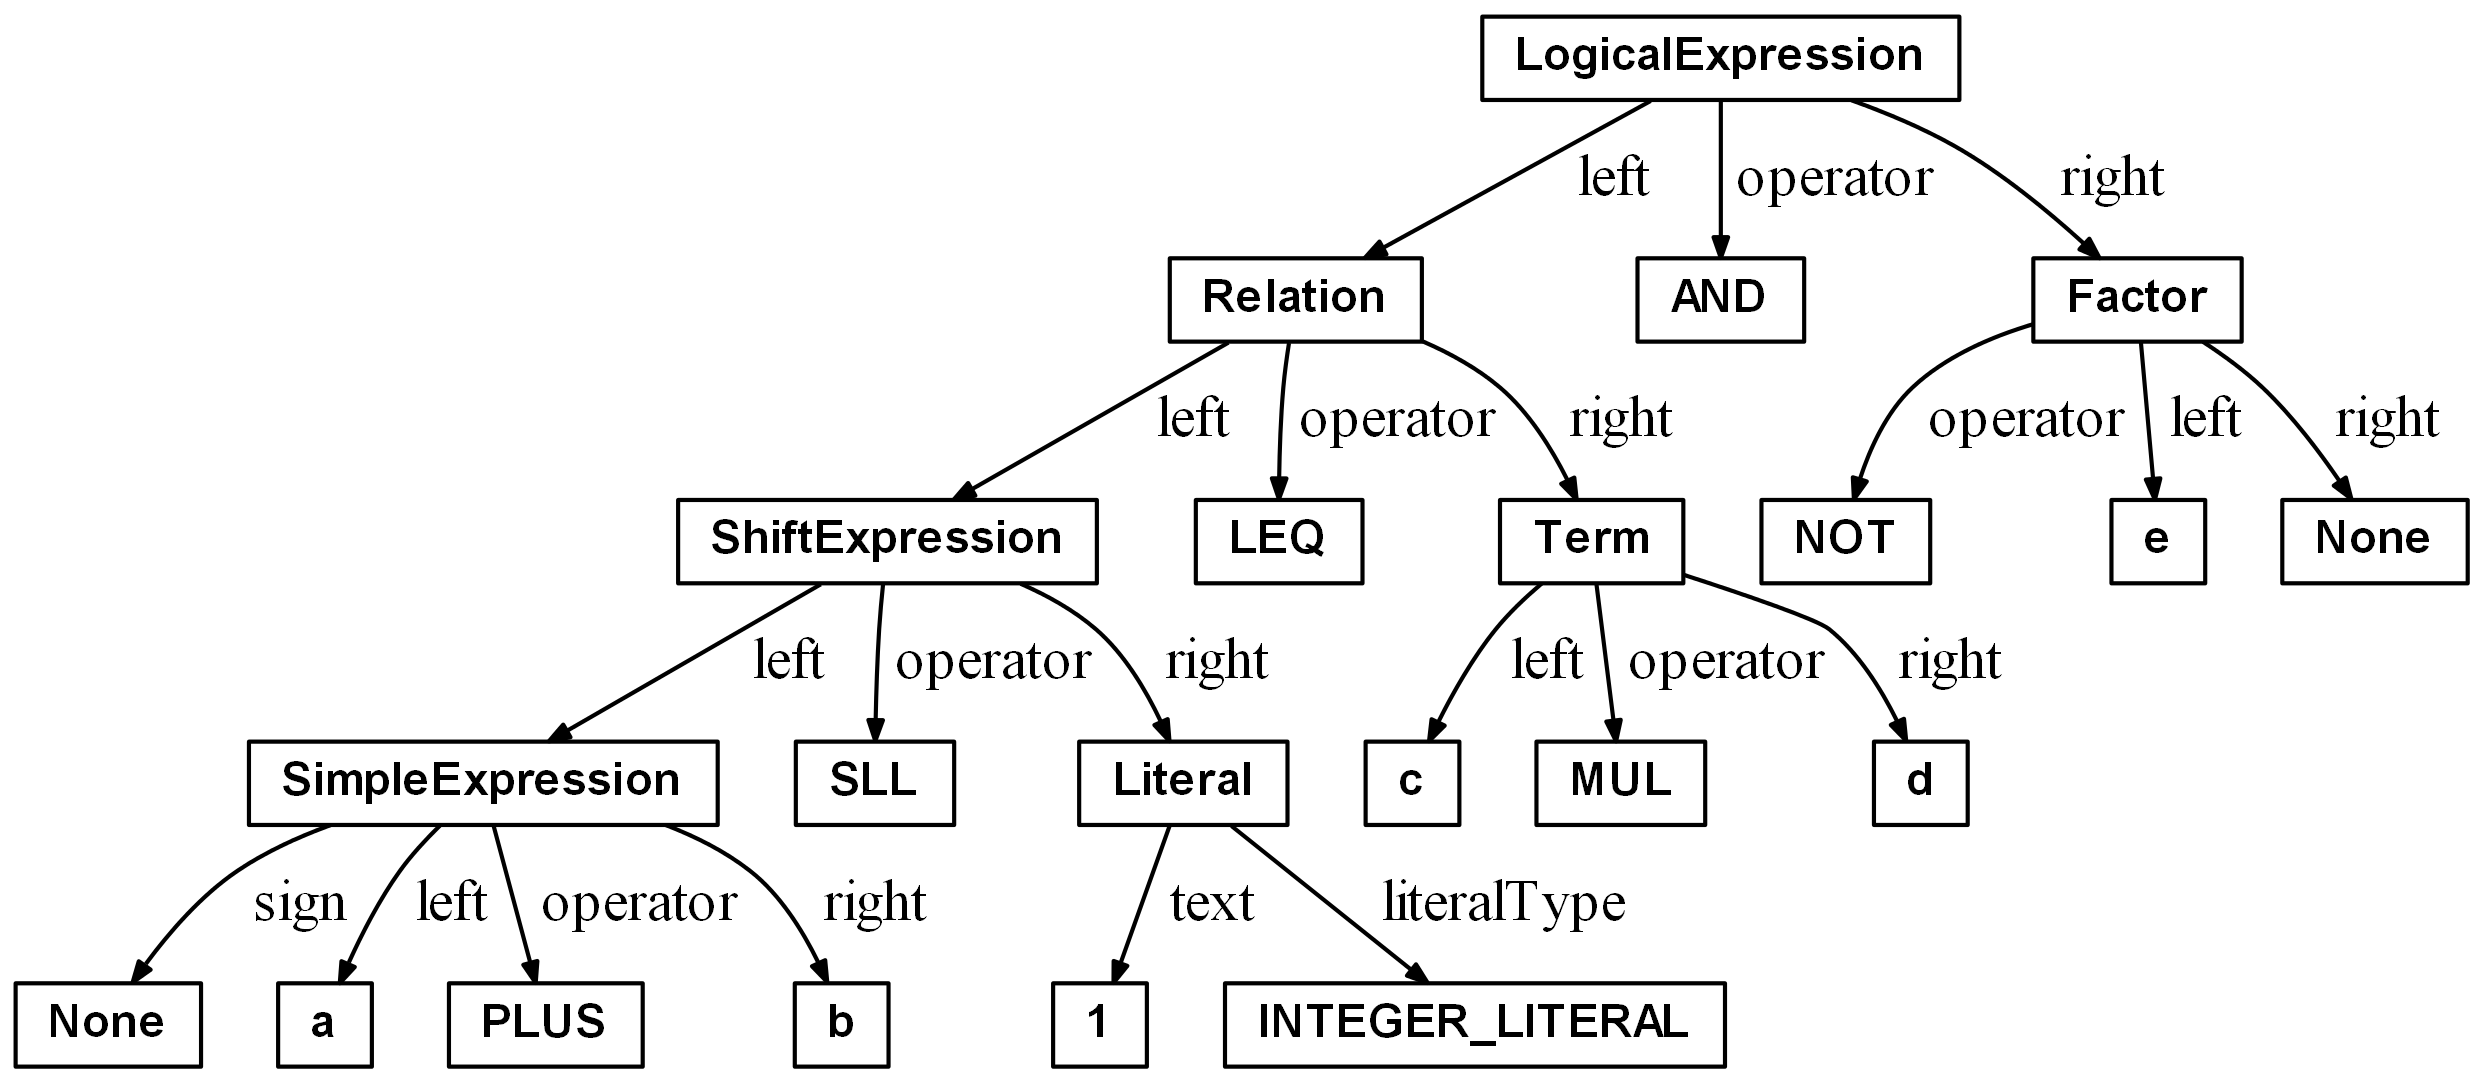
\includegraphics[scale=0.6]{images/LogicalExpression.png}
    \caption{AST-Knoten f�r eine Logical-Expression}
\end{figure}
Eine Logical-Expression besteht wie alle Binary-Expression aus einer linken und rechten Expression und einem Operator der beide miteinader verkn�pft.

\subsubsection{ConstantDeclaration}
\lstset{caption={}}
\lstinputlisting{src/ConstantDeclaration.vhd}
\begin{figure}
  \centering
    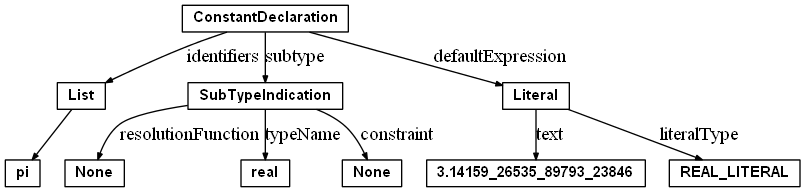
\includegraphics[scale=0.6]{images/ConstantDeclaration.png}
    \caption{AST Knoten f�r eine Constant-Declaration}
\end{figure}
Die Deklaration f�r eine Konstante besteht aus einer Liste von Identifiers, einer Type Beschreibung und einem Default-Wert.

\subsection{AST Manipulation}
\todo{Text}
\section{Symboltabelle}
\section{Codeerzeugung}